\chapter{Background}
\label{chap:background:intro}

In this chapter the following concepts will be introduced and explored to
provide the necessary context for the remaining chapters in this thesis. First
convolutional neural networks will be introduced along with a mathemtaical
representation of the convolution operation. Afterwhich, different ways to
compute the convolution operation will be discussed. Then a methodology for
analysing convolution operation accelerators will be examined, specifically an
approach to thinking about a convolution accelerator's dataflow design space as
well as it's hardware design space will be presented. Finally this chapter
concludes with a discussion of related work in the literature. 


\clearpage

\section{Convolutional neural networks and the convolution operation}
\label{chap:background:cnns_and_conv}

Nerual networks are a class of machine learning models used for various tasks
like image recognition and object detection. They can be trained to model
complex mathematical functions. Neural networks are characterized by the
different layers used in them to compute some expected output from an input.
Convolution neural networks are then characteried by the emphasis on the use of
the convolution layer in computing the networks output. In addition to
convolution layers, CNNS commonly make use of other layer types like fully
connected layers as well activation and batch normalization layers
however the bulk of a networks runtime is spent computing these convolution
layers \cite{most_of_the_runtime}. There are many different variants of the
convolution operation used in the convolution layer. Some convolution layer
variants use sparse weights. Others like grouped and depthwise convolution
layers change the input and output channel relationship to reduce the number of
multiply and accumulate operations required for the layer. An illustration of a
the different layers that can be present in a CNN is presented in
\autoref{fig:cnn_network}

\begin{figure}[ht]
    \centering
    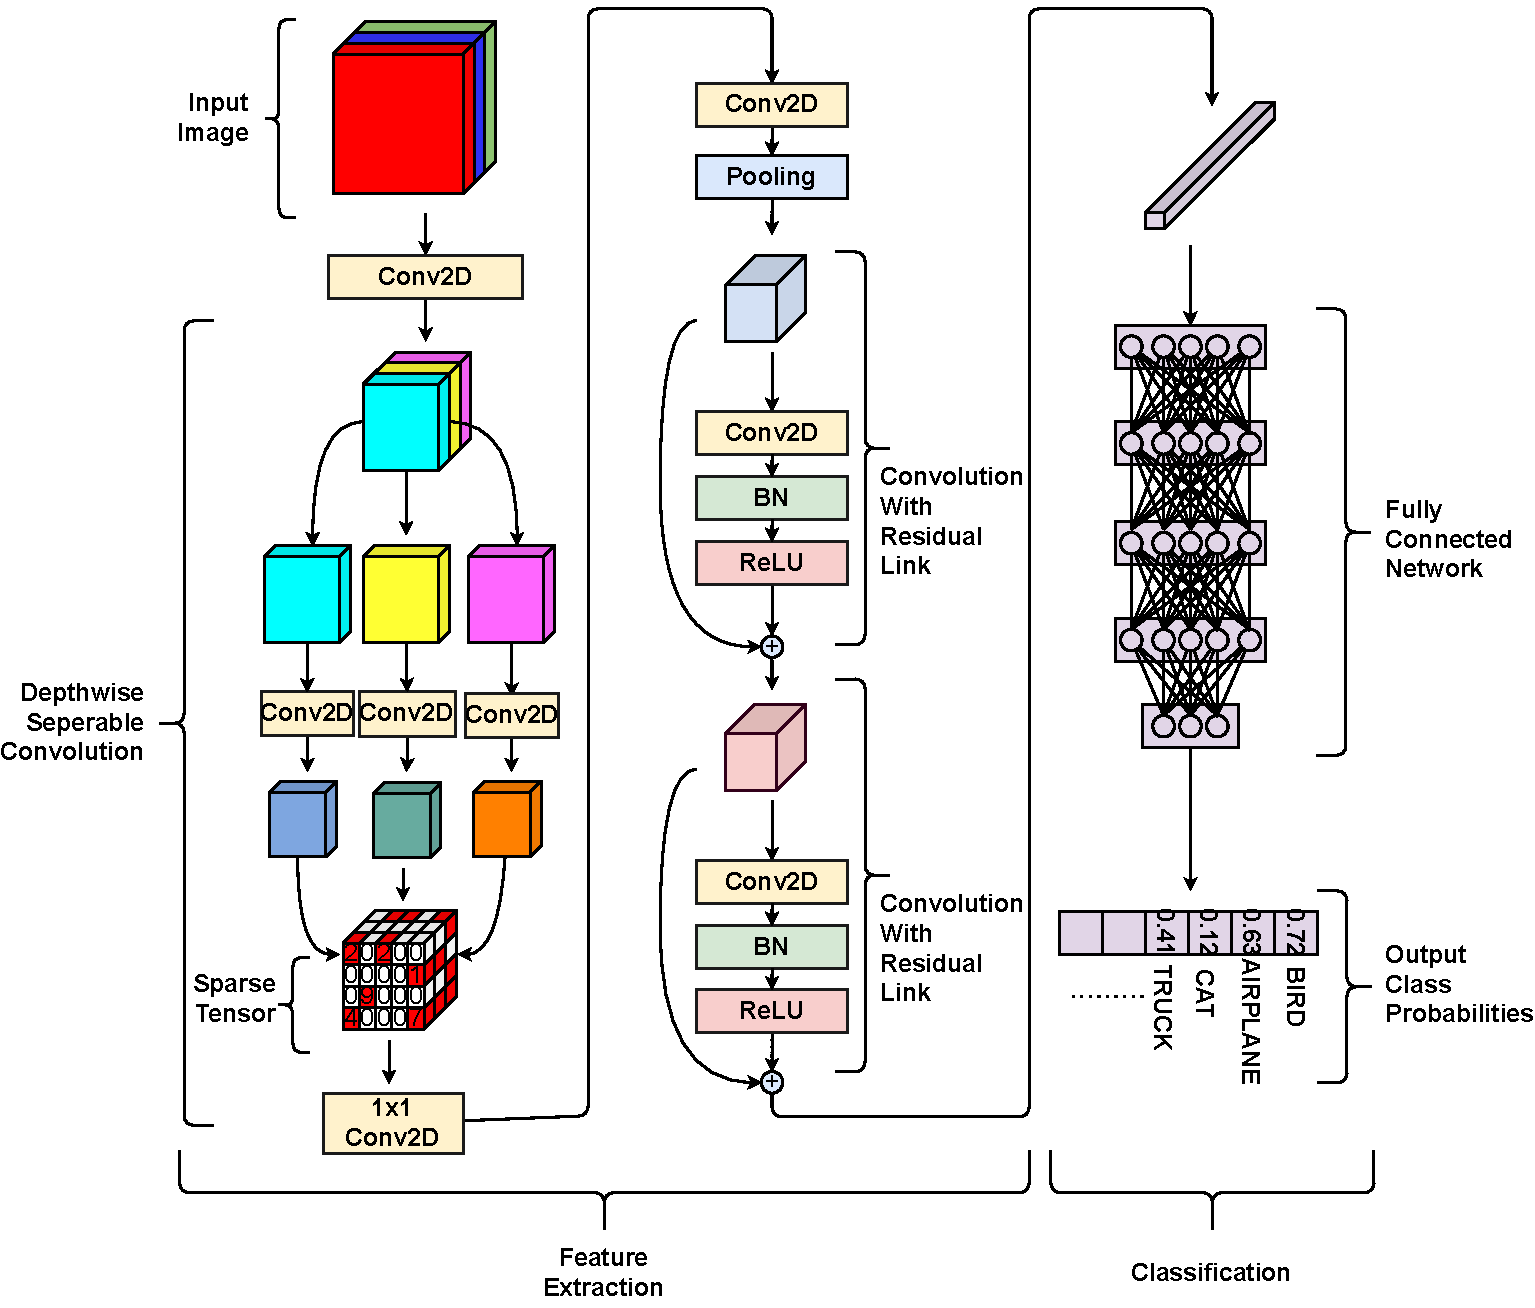
\includegraphics[scale=0.4]{fig/cnn.pdf}
    \caption0{Example of the different layers in a convolution neural networks}
    \label{fig:cnn_network}
\end{figure}


Assuming the input feature map, output feature map and weight dimentionalities
of a layer are defined in \autoref{math:default_tensor_def}. A mathematical
representation of the convolution is given in \autoref{math:conv_equation_1fp}.
\autoref{math:conv_equation_1fp} represents a stencil based operation were a
sliding window called a kernel is moved accross an input feature and at each
position a multiply and accumulate operation is performed to compute an output
element of the output feature map. This stencil operation is repreated for each
kernel present in the layer. The number of kernels in a layer is called the
number of filters. This multiply and accumulate operate occurs accross the all
three dimensions of the IFmap tensor. In addition to the mathematical
description in \autoref{math:conv_equation_1fp} a visual representation of the
convolution operation is given in \autoref{fig:conv_explained}. 


\begin{align}
    \begin{split}
        IFmap \in R^{C \times n\times n} \\
        OFmap \in  R^{F \times m\times m} \\
        Weight \in R^{F \times C\times K\times K} \\
    \end{split}
    \label{math:default_tensor_def}
\end{align}

\begin{align}
    OFmap[f][y][x] = \displaystyle\sum\limits_{c=0}^{C-1}\displaystyle\sum\limits_{k_x=0}^{K-1}\displaystyle\sum\limits_{k_y=0}^{K-1}Weight[f][c][k_y][k_x]*IFmap[c][y+ky][x+kx]
    \label{math:conv_equation_1fp}
\end{align}


\begin{figure}[ht]
    \centering
    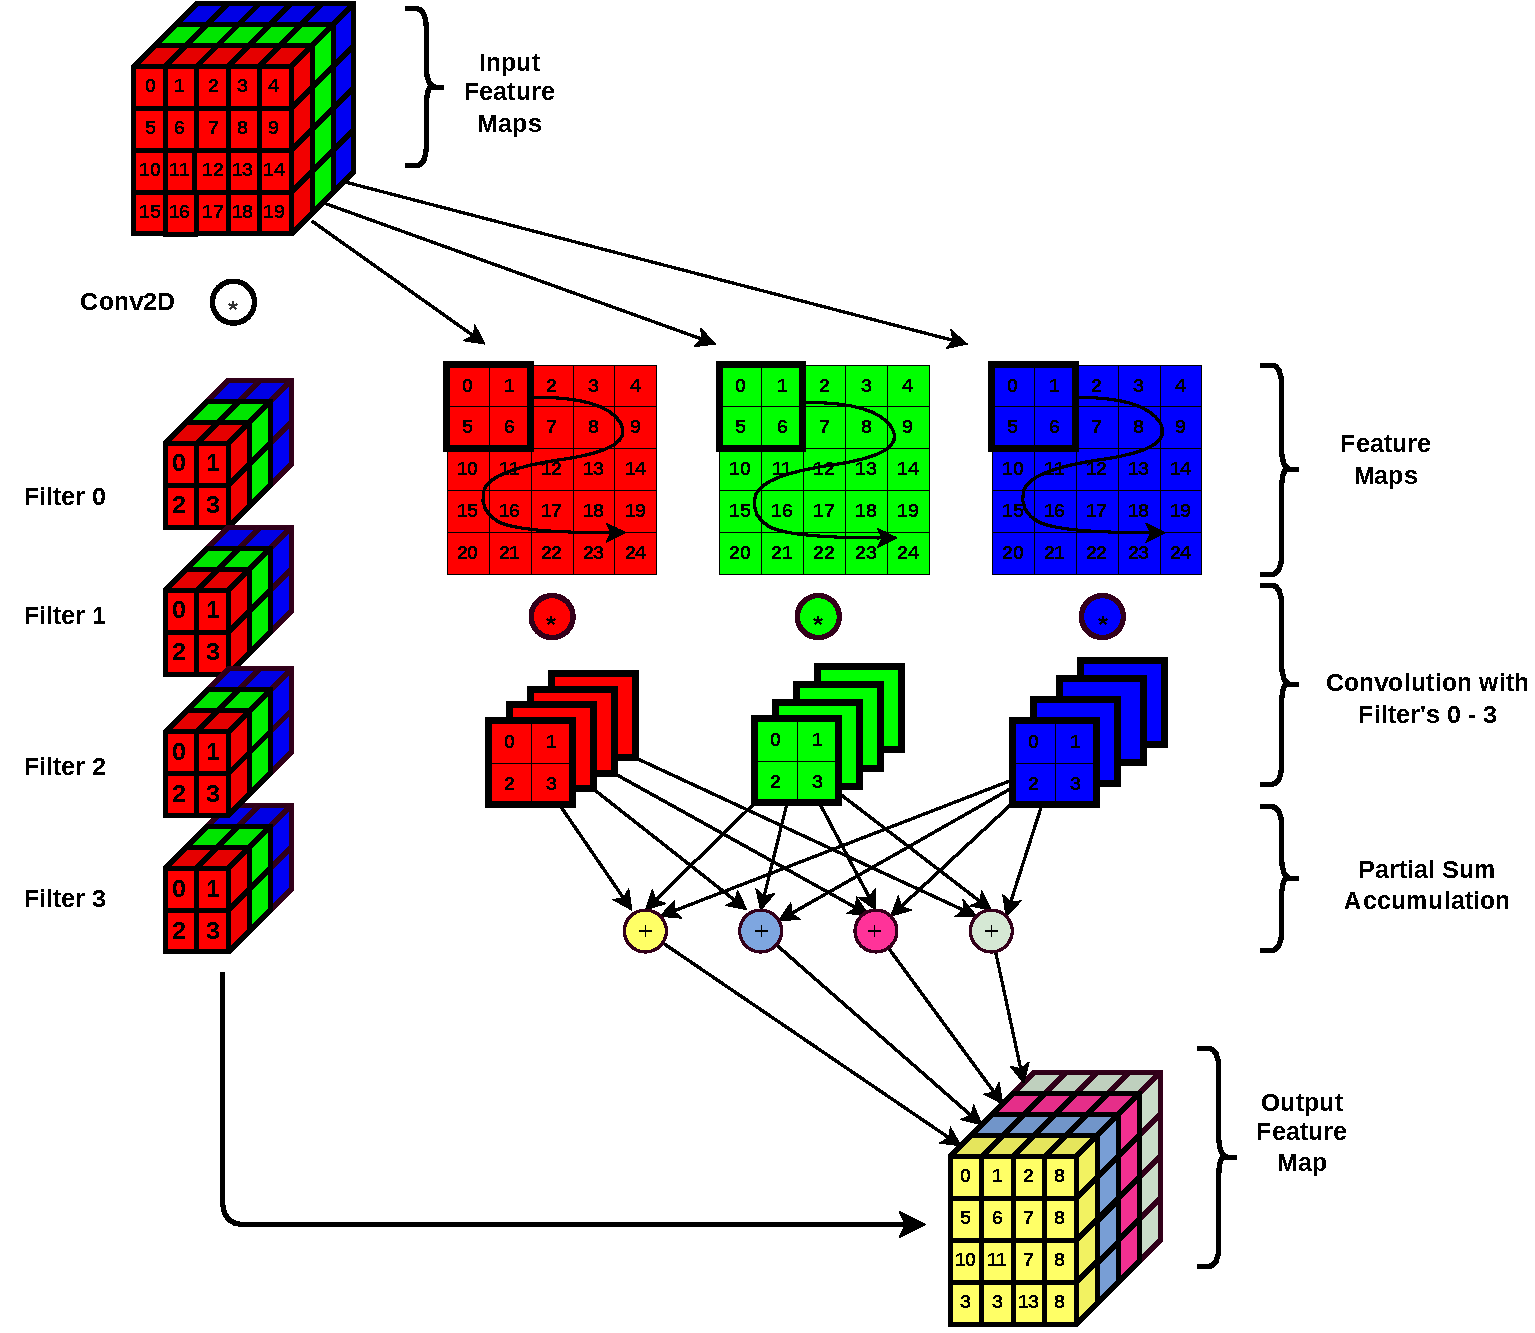
\includegraphics[scale=0.6]{fig/ConvExplained.pdf}
    \caption{Convolution Operation Illustrated}
    \label{fig:conv_explained}
\end{figure}

\section{Computing the convolution operation}
\label{chap:background:cnns_and_conv}

Direct naive implementation of \autoref{math:conv_equation} with tensors
\autoref{math:default_tensor_def} as a series of loops is given below
\autoref{lst:conv_loop}

\begin{minipage}{\linewidth}
    \begin{lstlisting}[language=C, caption=Convolution implemented as nested loops, label={lst:conv_loop}]
for(int f = 0; f < F; f++) // Filter loop
    for(int c = 0; c < C; c++) // Channel loop
        for(int y = 0; y < Y; y++) // Output feature map row
            for(int x = 0; x < X; x++)  // Output feature map col
                for(int ky = 0; ky < KY; ky++)  // Kernel row
                    for(int kx = 0; kx < KX; kx++)  // Kernel col
                        O[f][y][x] += I[c][y+ky][x+kx]*W[f][c][ky][kx];
    \end{lstlisting}
\end{minipage}

\newpage

\section{Convolution as general matrix multiplication}
\label{chap:intro:conv_operation}

\begin{figure}[ht]
    \centering
    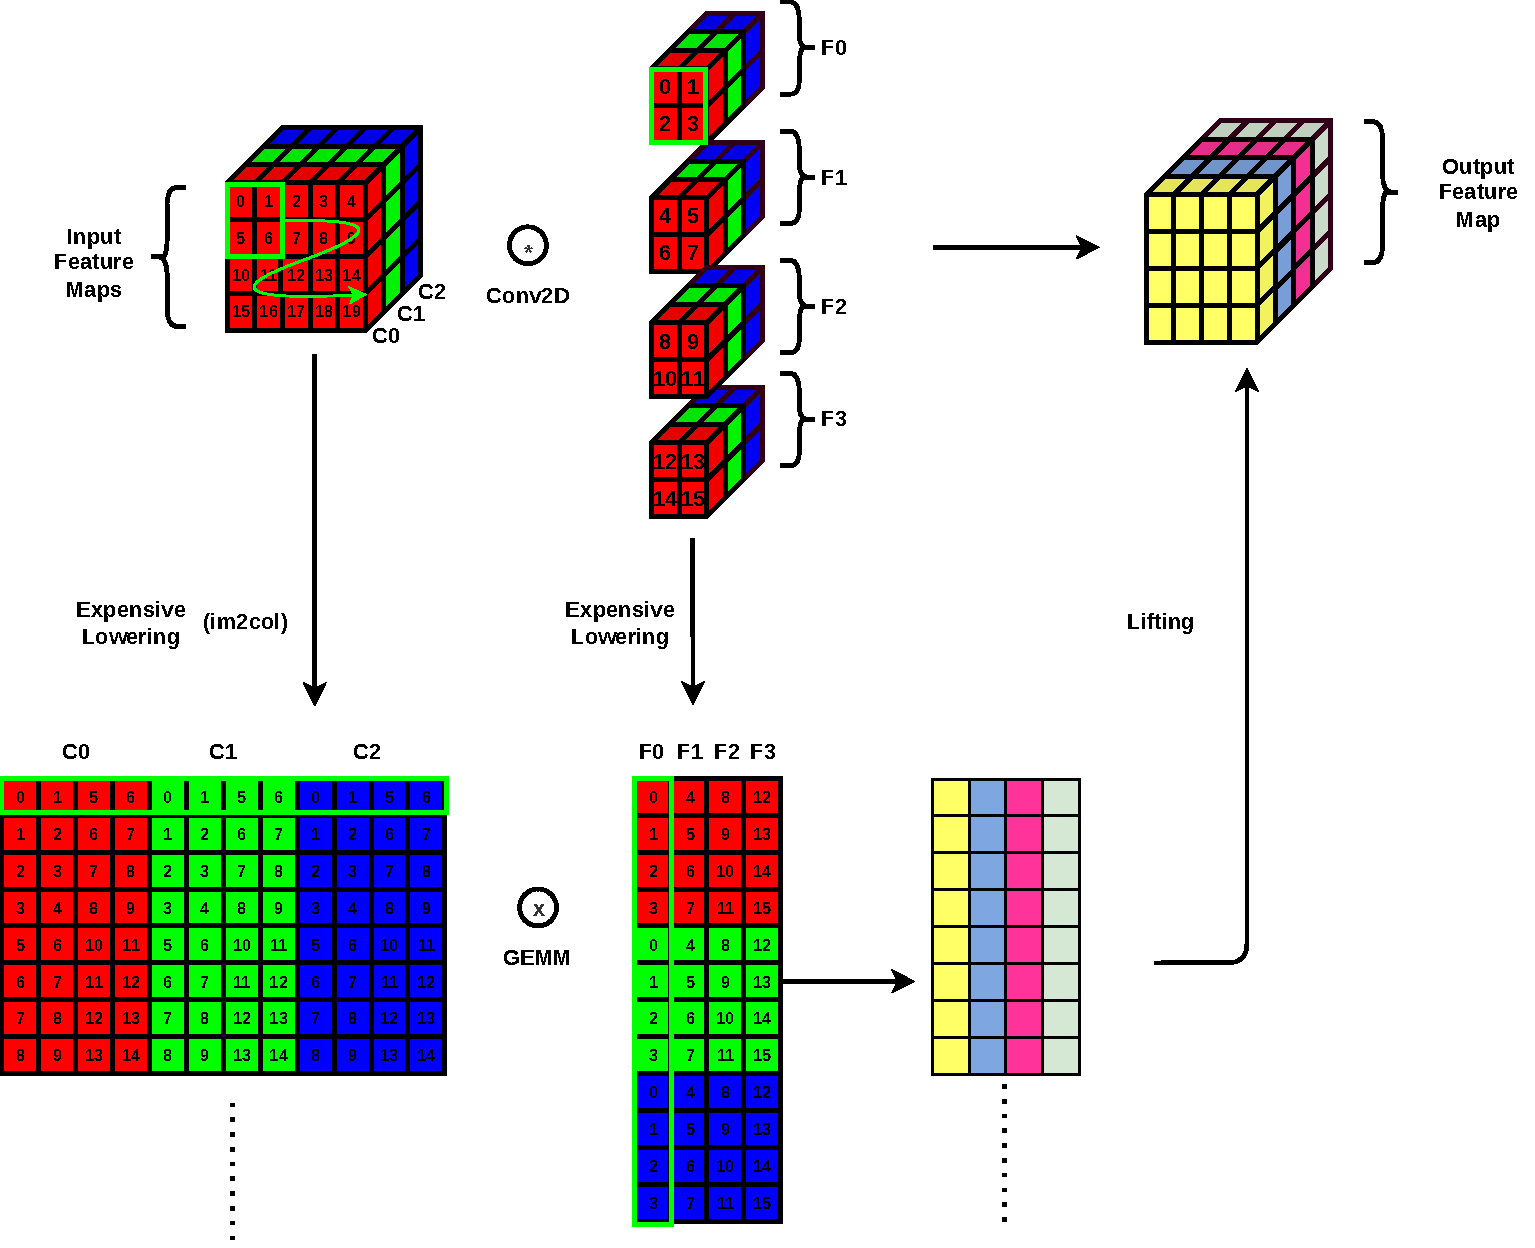
\includegraphics[scale=0.6]{fig/Im2Col.pdf}
    \caption{Im2Col Illustrated}
    \label{fig:im2col}
\end{figure}

Convolution can be converted into a \ac{GEMM}

Popular techniques like im2col (illustrated in \autoref{fig:im2col}) can be used
to convert any convolution operation into \ac{GEMM} (listed as expensive
lowering \cite{cafe_con_troll}) but there are others techniques that don't
produce such massive input feature maps


If willing to increase complexity of lowering of ifmap and weight tensors after
GEMM we can reduce bloat in ifmap with balanced lifting/ loading in
\cite{cafe_con_troll}. Analytical expressions adapted from \cite{cafe_con_troll}
are given below with the inclusion of lowering in the presence of multiple
filters.


\clearpage

\begin{align}
    \begin{gathered}
        IFmap \in R^{C\times n\times n} \xrightarrow[]{Balanced Lowering} \hat{IFmap} \in R^{nm\times KC} \\
        \hat{IFmap}[cn+r, :] = vec(IFmap[:, r, c:c+K]) \\
        \forall r,c \in [0, n-1], [0, m-1]
    \end{gathered}
    \label{math:balanced_lowering_ifmap}
\end{align}

\begin{align}
    \begin{gathered}
        Weight \in R^{F\times C\times K \times K} \xrightarrow[]{Balanced Lowering} \hat{Weight} \in R^{KC\times FK}\\
        \hat{Weight}[f*K:f*K+K, i] = vec(Weight[f, :, i, :]) \\
        \forall f,i \in [0, F-1], [0, K-1]
    \end{gathered}
    \label{math:balanced_lowering_weight}
\end{align}
In balanced lowering, we first lower the ifmap and weights using expression 
\eqref{math:balanced_lowering_ifmap} and \eqref{math:balanced_lowering_weight}.

\begin{align}
    \begin{gathered}
        \hat{OFmap} = \hat{IFmap}.\hat{Weight}
    \end{gathered}
    \label{math:balanced_lowering_gemm}
\end{align}
Then a \ac{GEMM} is performed \eqref{math:balanced_lowering_gemm}


\begin{align}
    \begin{gathered}
        \hat{OFmap} \in R^{nm\times FK} \xrightarrow[]{Balanced Lifting} OFmap \in  R^{m\times m\times F}\\
        OFmap[f, r, c] = (\displaystyle\sum\limits_{j=0}^{K-1} \hat{OFmap}[cn+r+j, j+fK]) \\
        \forall f,r,c \in [0, F-1], [0, m-1], [0, m-1]
    \end{gathered}
    \label{math:balanced_lifting_ofmap}
\end{align}

Followed by a lift operation on the output $\hat{OFmap}$ matrix using \eqref{math:balanced_lifting_ofmap}

Illustration of this data transformation is presented in \autoref{fig:balanced_lowering_lifting}

Pros of lowering/ lifting

Conv as GEMM Offers the most flexibility because it’s insensitive to changes in
convolution parameters

It also allows leaves us with a GEMM accelerator which is useful for many other
NN layers e.g Linear/ Self attention/ LSTM

Con is that it still causes bloat in ifmap and additionaly complexity/ latency of 
lifting/ lowering. Which in the balanced case is $m^{2}K$ \cite{cafe_con_troll}

\begin{figure}[!ht]
    \centering
    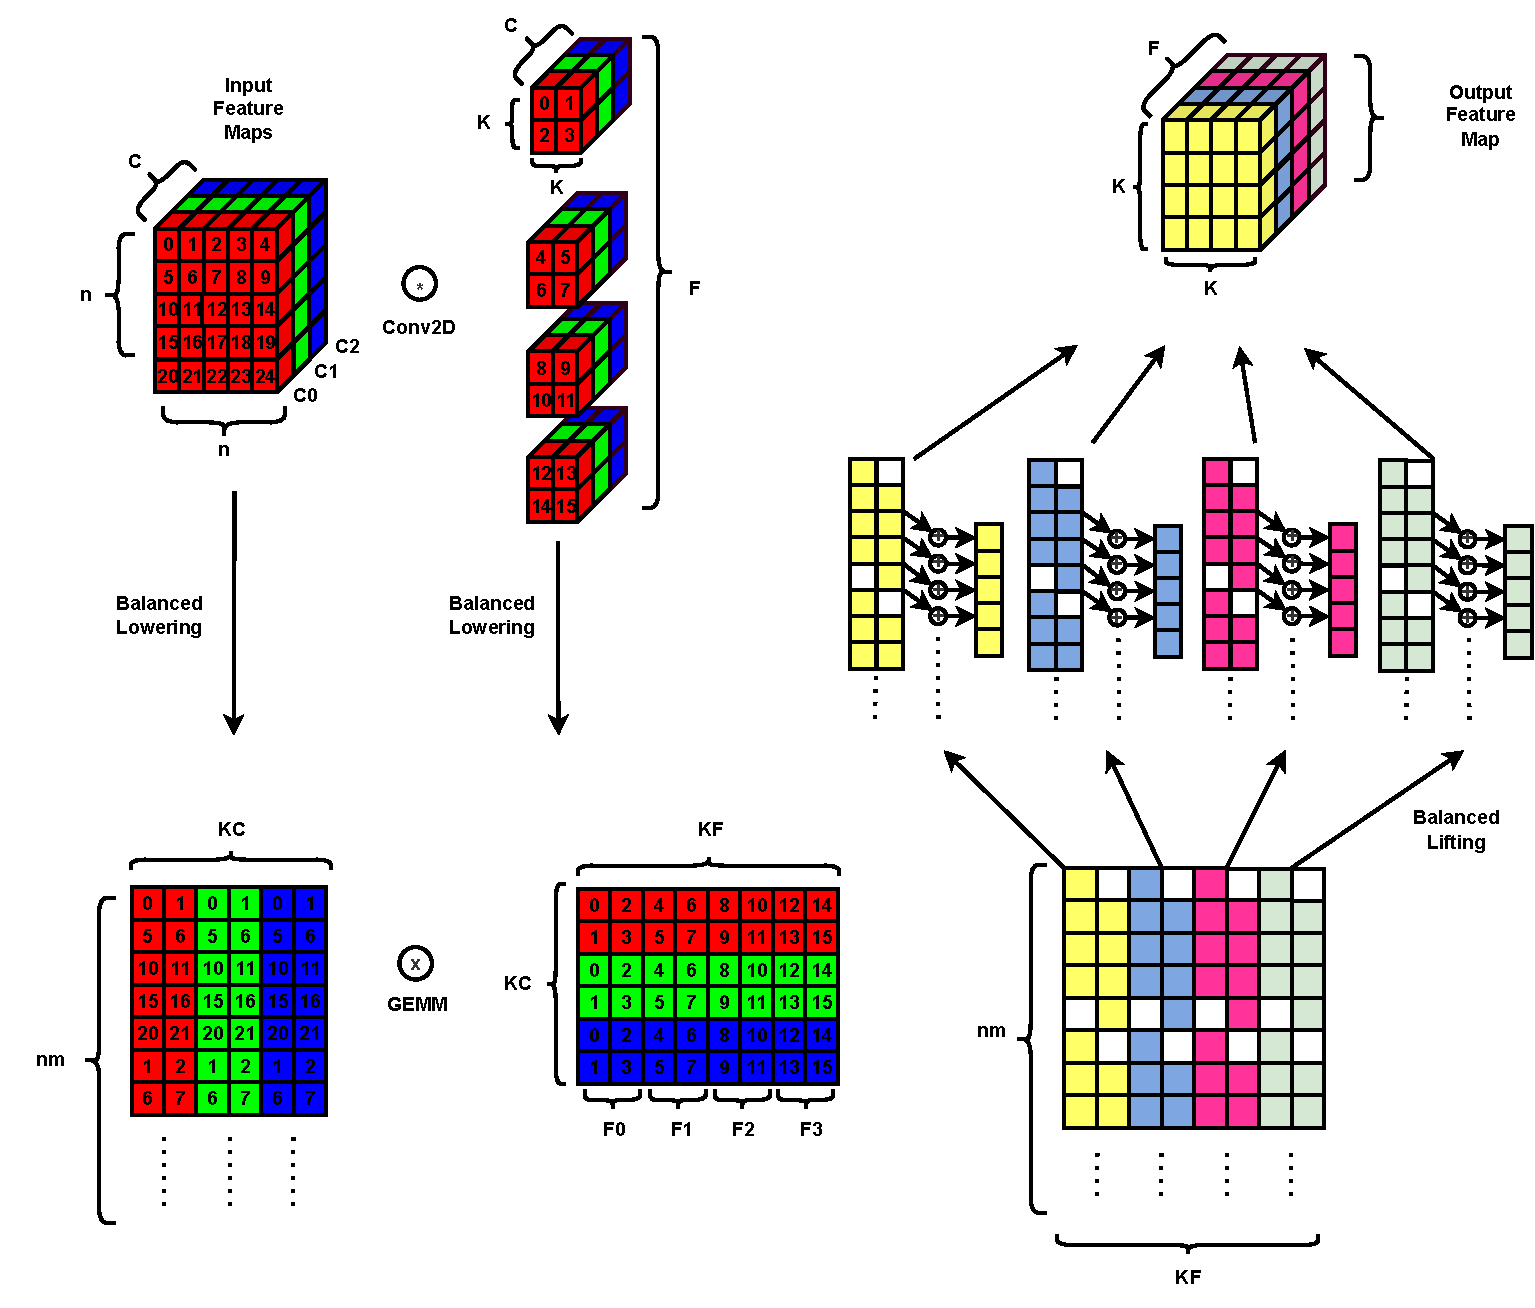
\includegraphics[scale=0.6]{fig/BalancedLoweringLifting.pdf}
    \caption{Balanced Lowering/Lifting Illustrated}
    \label{fig:balanced_lowering_lifting}
\end{figure}


\section{Implementing convolutions in hardware}
\subsection{The dataflow taxonomy}

In the dataflow design space, from \cite{dnn_df_overrated} 
dataflows can be represented using the direct convolution
nested loop structure combined with unroll pragmas. Listing \ref{lst:W_S_Generic_Loop} shows a generic
implementation of a single convolution layer as a loop structure under a weight
stationary dataflow configuration. What defines that dataflow is 1) loop unroll
targets 2) loop order 3) the unroll factors of the unrolled loops. Weight elements within a
kernel remain stationary throughout the computation of an output feature map
until a new tile of channels C\_T is loaded into the accelerator. Once the
weights within a particular channel and filter group are used to produce an
output feature map they are discarded and are only loaded again when computing
the same layer for a new input image. From listing \ref{lst:W_S_Generic_Loop} we
can see that from the loop unroll targets and loop unroll factors there are many
other possible dataflow configurations available to us outside of weight
stationary. Additionally, since accelerators are generally limited to two
spatial axis the loops of the convolution operation can be mapped to two spatial
axis. If we allow multiple convolution loops under some kernel unroll factor
KY\_T/KX\_T  to be unrolled and mapped to the same accelerator spatial axis we
can influence the effective unroll factors when performing different
convolutions of different kernel sizes other than KY\_T/KX\_T. The choice of
which loops are mapped to which spatial axis is an additional design dimension
alongside loop unrolling. To summarize, from the loop representation of
convolution accelerator dataflows we have three design space dimensions, 1) Loop
unroll targets 2) Loop unroll factors 3) Loop spatial mapping. Given the size of
this dataflow design space we will use CIGAR and Tempo to derive the common
case for convolution layers and limit the scope of the dataflow design space.

CNN layer loops + loop ordering + Loop tilings can express different
accelerators dataflows like row stationary, weight stationary, etc



\begin{minipage}{\linewidth}
    \begin{lstlisting}[language=C, caption=Convolution implemented as nested loops, label={lst:conv_loop}]
#pragma UNROLL F_T
for(int f = 0; f < F; f+=F_T) // Filter loop
#pragma UNROLL C_T
    for(int c = 0; c < C; c+=C_T) // Channel loop
#pragma UNROLL Y_T
        for(int y = 0; y < Y; y+=Y_T) // Output feature map row
#pragma UNROLL X_T
            for(int x = 0; x < X; x+=X_T)  // Output feature map col
#pragma UNROLL KY_T
                for(int ky = 0; ky < KY; ky+=KY_T)  // Kernel row
#pragma UNROLL KX_T
                    for(int kx = 0; kx < KX; kx+=KX_T)  // Kernel col
                        O[f][y][x] += I[c][y+ky][x+kx]*W[f][c][ky][kx];
    \end{lstlisting}
\end{minipage}


\begin{figure}
    \centering
    \subfigure[]{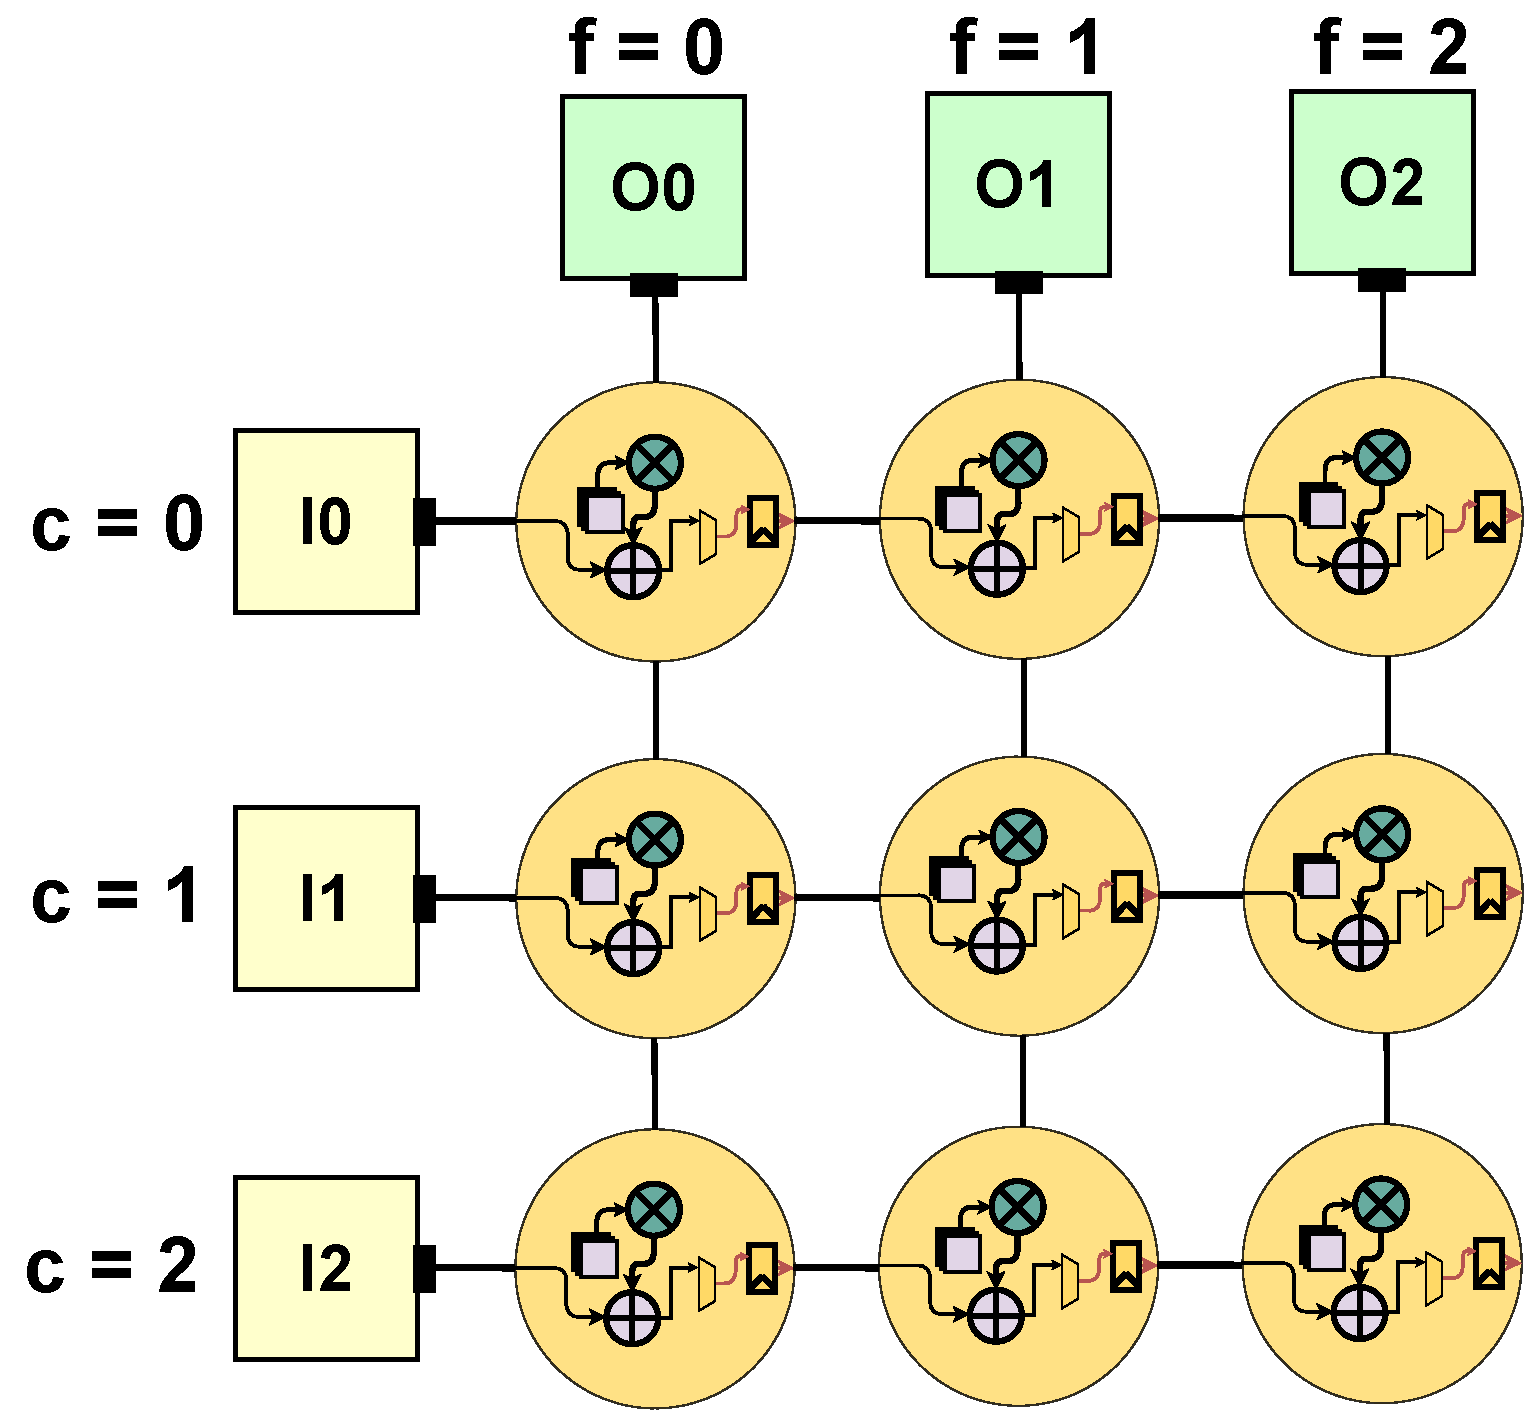
\includegraphics[width=0.32\textwidth]{fig/unroll_c_f.pdf}}
    \hspace{0.1cm} 
    \subfigure[]{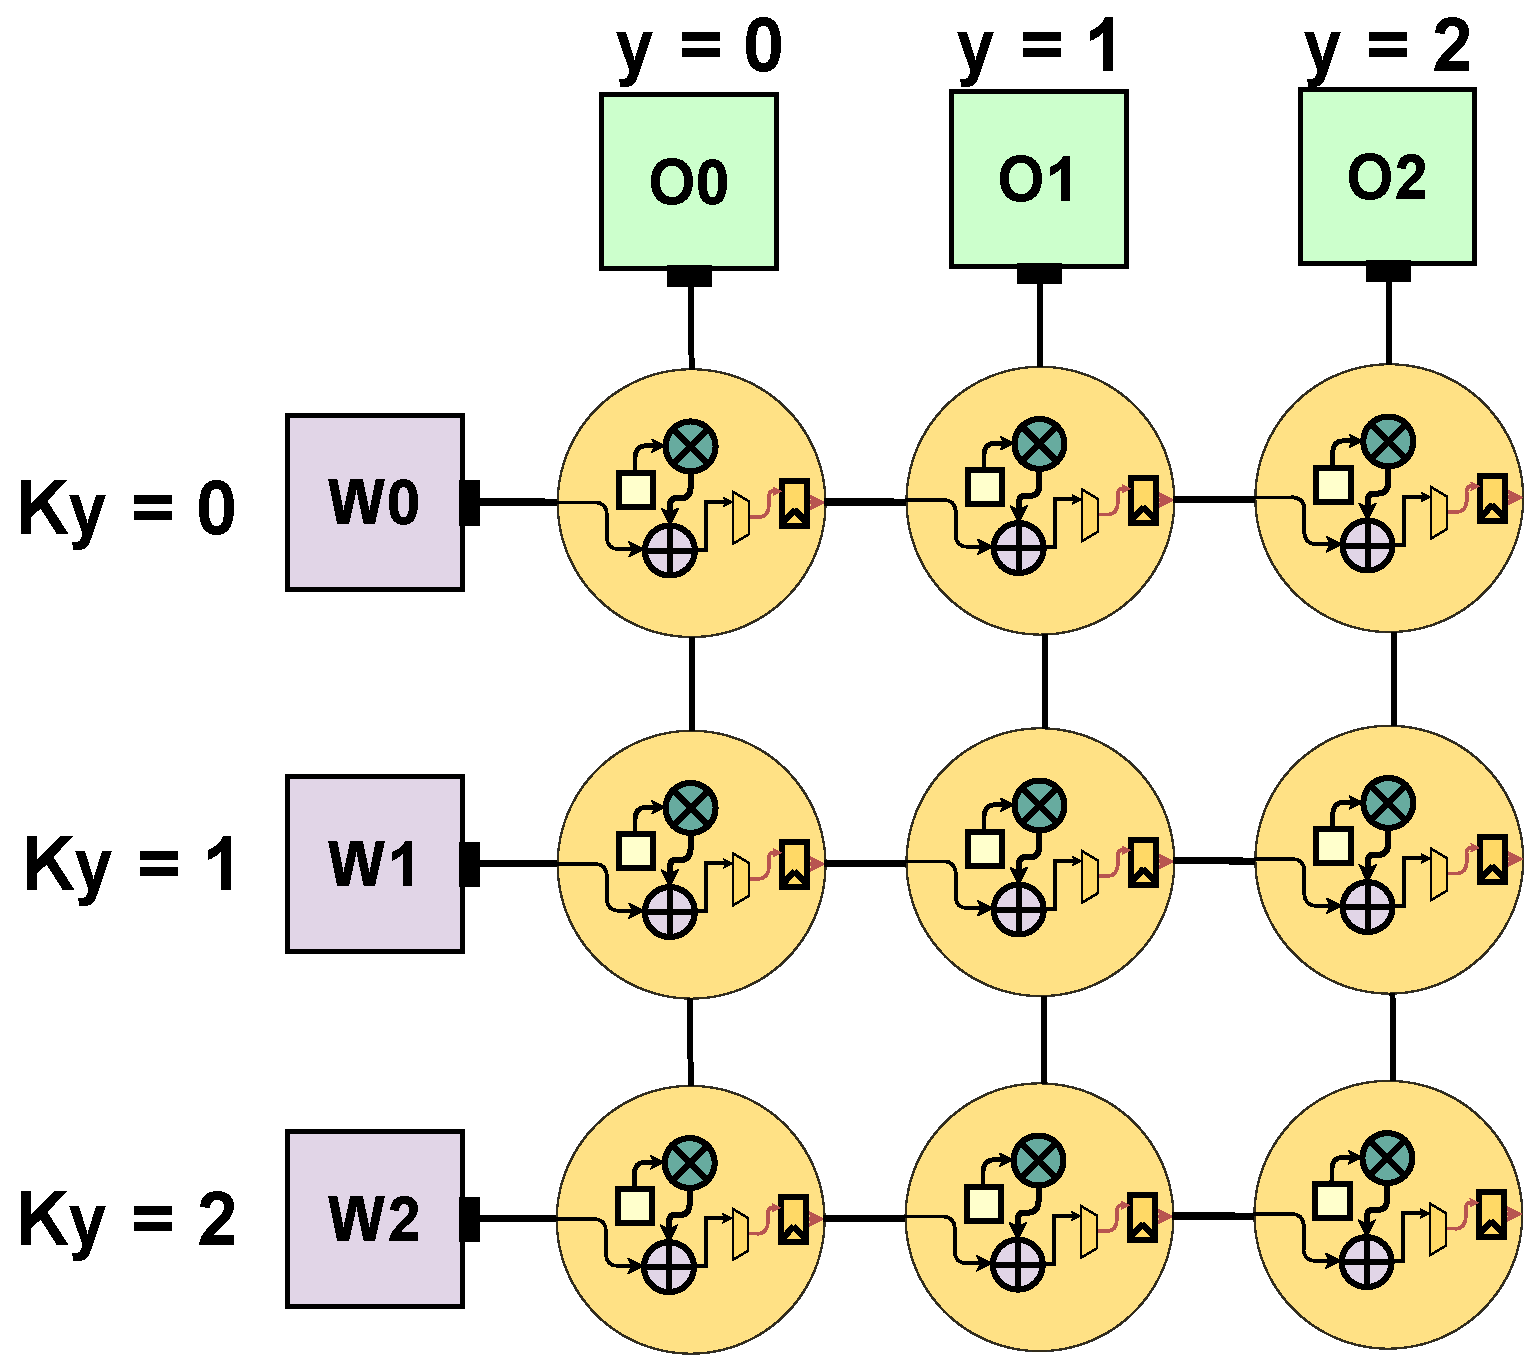
\includegraphics[width=0.32\textwidth]{fig/unroll_fy_y.pdf}}
    \hspace{0.1cm} 
    \subfigure[]{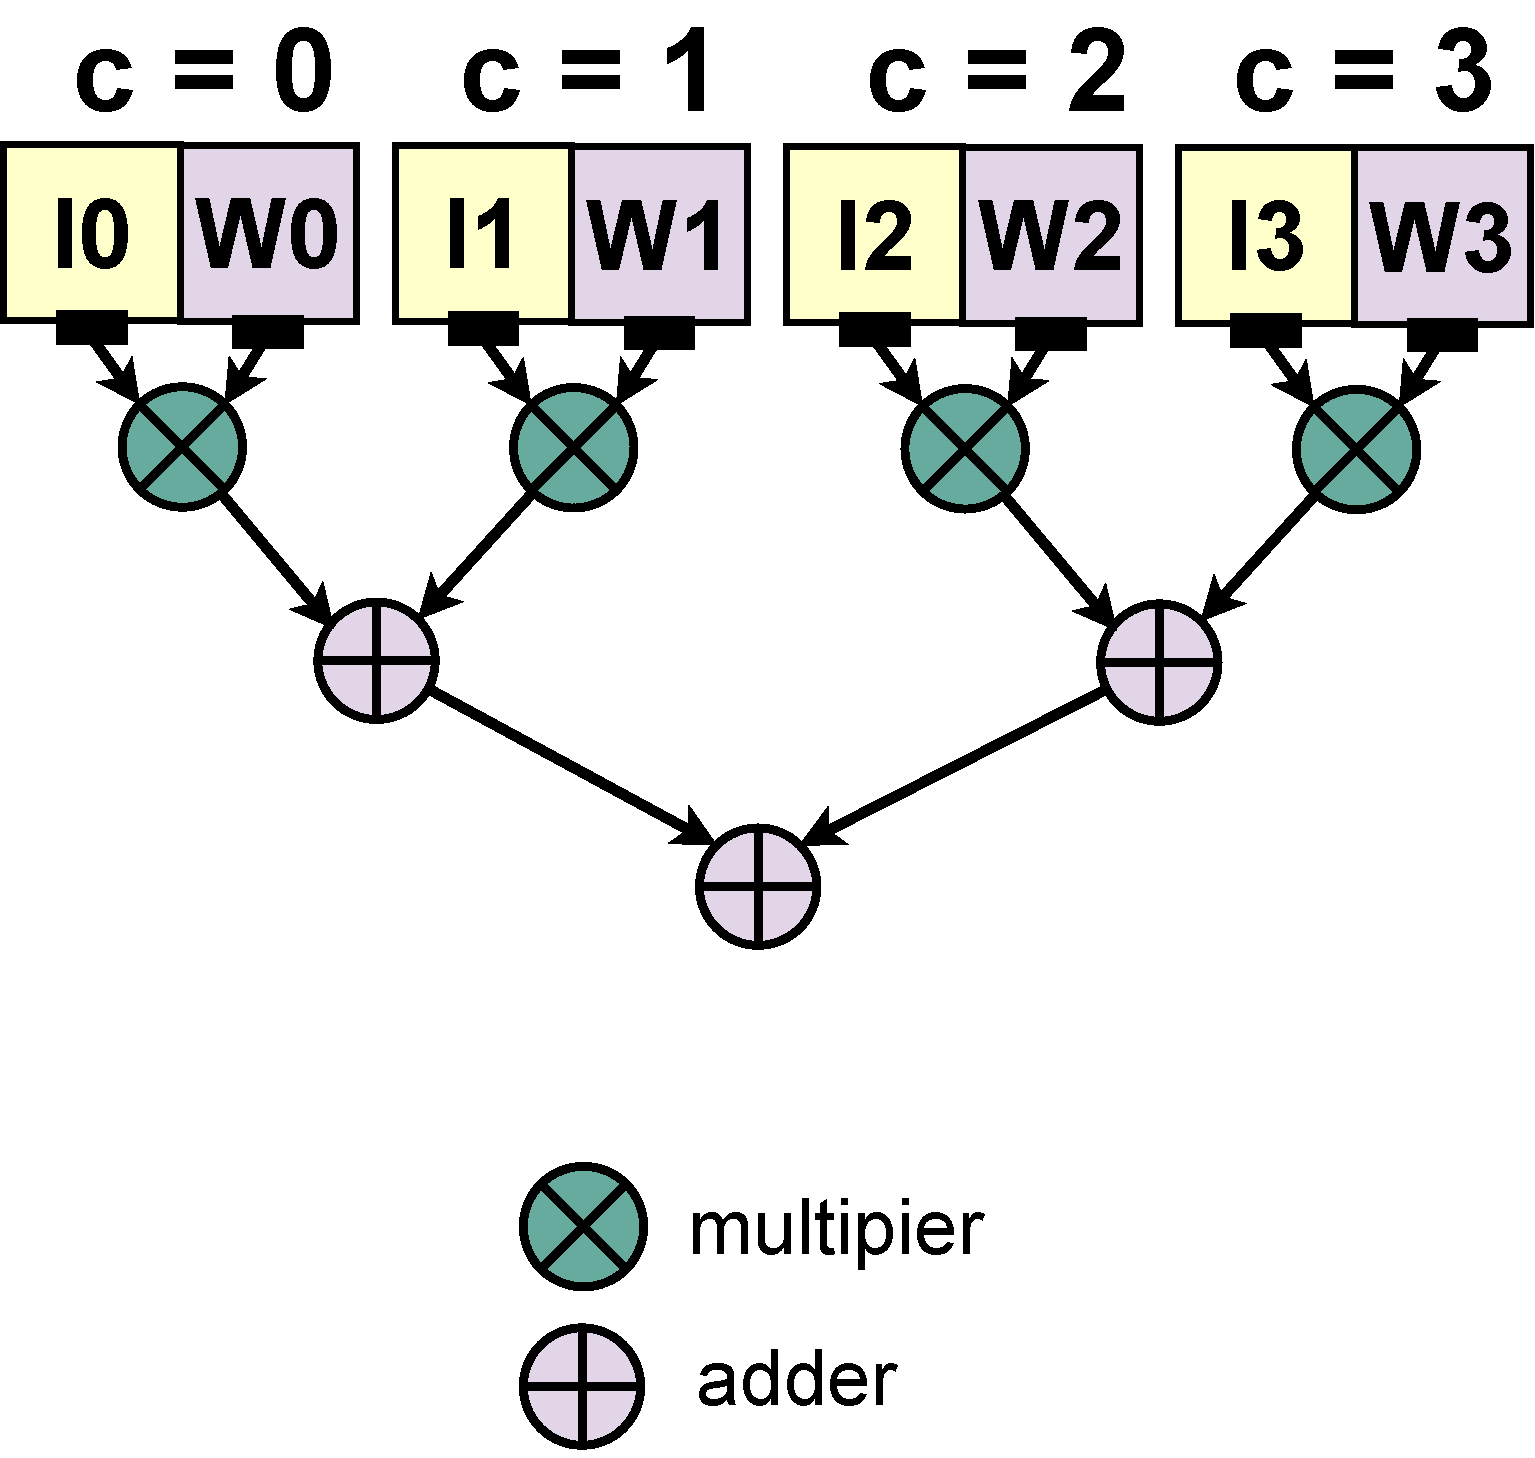
\includegraphics[width=0.32\textwidth]{fig/unroll_c.pdf}} 
    \hspace{0.1cm} 
    \subfigure[]{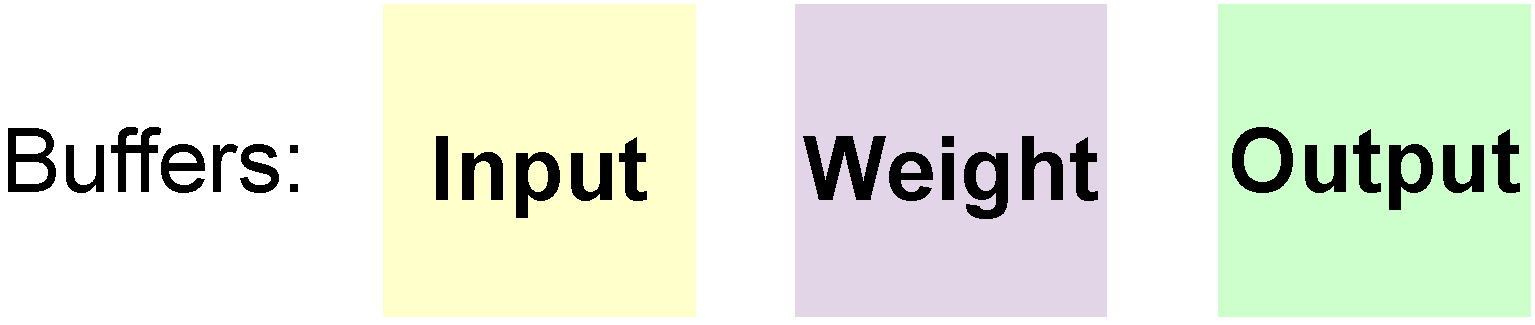
\includegraphics[width=0.3\textwidth]{fig/buffer_description.pdf}}
    \caption{Illustration of different dataflow implementations adapted from \cite{dnn_df_overrated} (a) blah (b) blah (c) blah (d) blah}
    \label{fig:unroll_illustration}
\end{figure}


From dataflow we can derive hw implementation based on communication pattern and
reuse behavior of the individual data elements accessed in the convolution
layer.

\subsection{The Hardware Implementation taxonomy}

Figures in \autoref{fig:unroll_illustration} show different reduction/ multicast
schemes based on reuse behavior of data elements (IFmap, OFmap, Weights)
apparent in the dataflow. The space of available schemes is not limited to those
presented in \autoref{fig:unroll_illustration} though. In \cite{maestro} a
hardware taxonomy illustrated in figure \autoref{fig:hw_taxonpmy}.

\begin{figure}[ht]
    \centering
    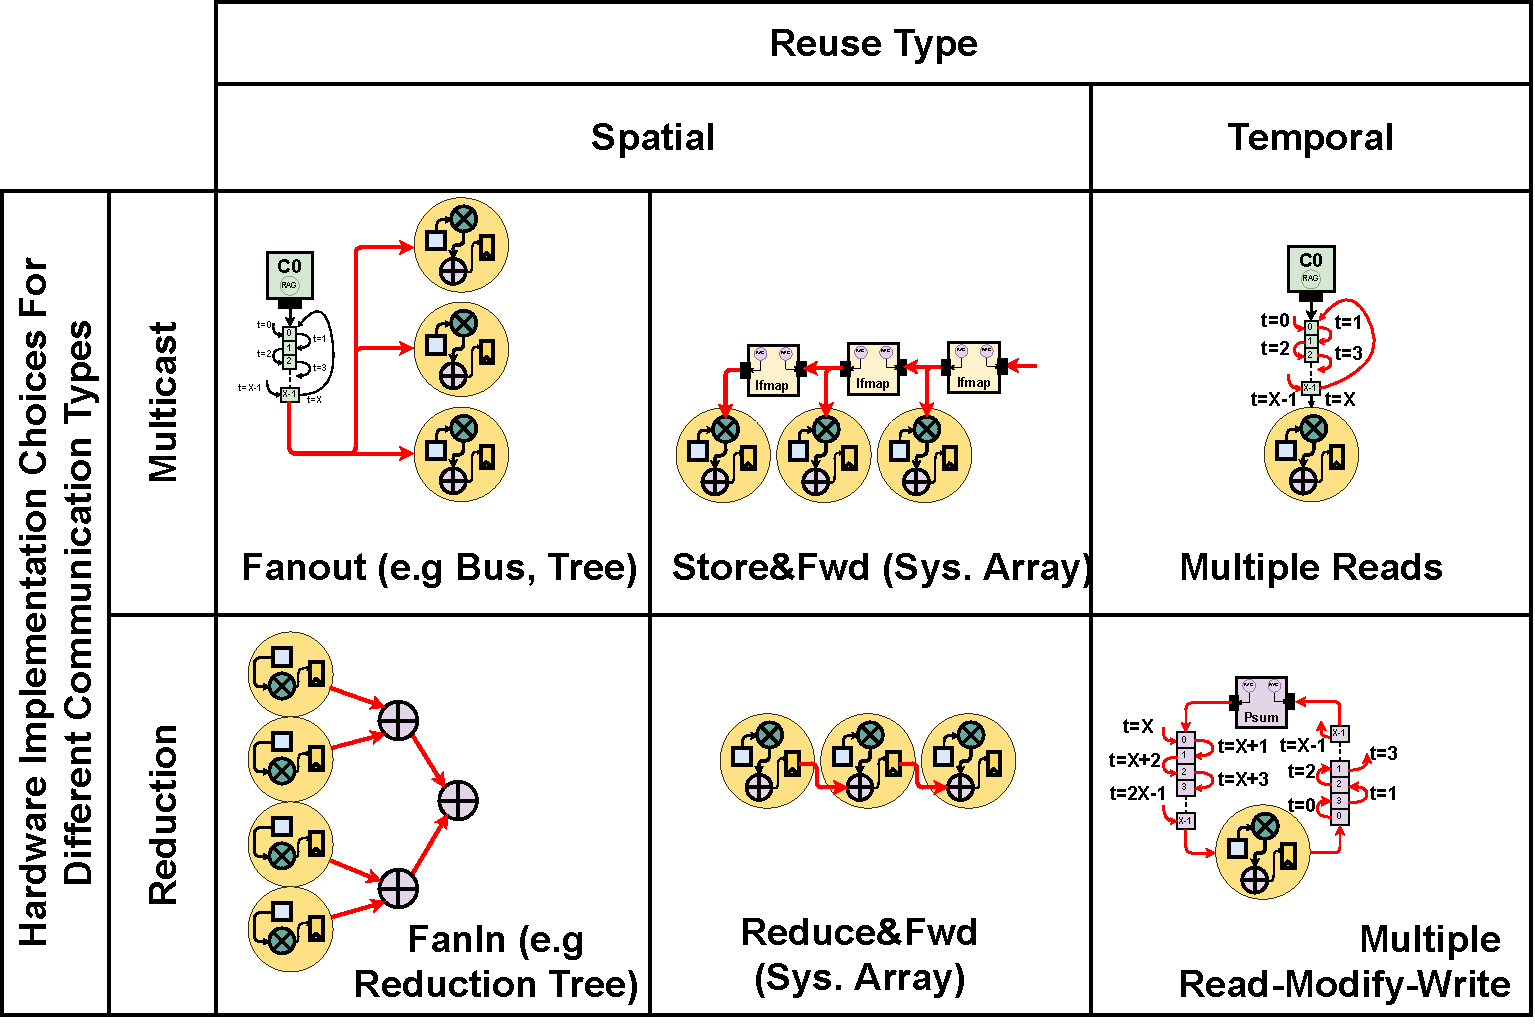
\includegraphics[scale=0.58]{fig/hw_taxonomy.pdf}
    \caption{Hardware Implementation Taxonomy adapted from \cite{maestro}}
    \label{fig:hw_taxonomy}
\end{figure}


Depending on the dataflow described using the dataflow taxonomy (1) loop
ordering (2) unroll targets (2) loop unroll factors. The implementation options
are derived based on the type of reuse present in the dataflow. Following the
hardware implementation taxonomy presented in in \cite{maestro}, we can classify
the available hardware implementation options based on the the type of reuse is
spatial (reuse distance = 0) or temporal (reuse distance > 0) that exists for a
given data element accessed in the dataflow. Within a reuse type, depending on
the nature of the reuse, if it is read or read modify write, there are several
options for supporting the communication inferred from the reuse. To deduce the
type of reuse and overall communicaiton behavior for each data element in any
dataflow we can use the polyhedral model to detect temporal reuse. Spatial reuse
detection can be inferred directly from the loops.


\section{Related work}
\label{chap:related_work}

\subsection{Convolution accelerator architectures}
 
TPU -> Pure GEMM
Eyeriss -> Emphasis on sparsity, no support for linear operations
Maeri -> Flexible mapping but we rely on optimizer rather than do it at runtime


\subsubsection{Eyeriss V1 and V2}

Eyeriss

Eyeriss is an accelerator for state-of-the-art deep
convolutional neural networks (CNNs). It optimizes for the energy
efficiency of the entire system, including the accelerator chip
and off-chip DRAM, for various CNN shapes by reconfiguring
the architecture. CNNs are widely used in modern AI systems
but also bring challenges on throughput and energy efficiency
to the underlying hardware. This is because its computation
requires a large amount of data, creating significant data
movement from on-chip and off-chip that is more energyconsuming than computation. Minimizing data movement energy
cost for any CNN shape, therefore, is the key to high throughput
and energy efficiency. Eyeriss achieves these goals by using a
proposed processing dataflow, called row stationary (RS), on a
spatial architecture with 168 processing elements. RS dataflow
reconfigures the computation mapping of a given shape, which
optimizes energy efficiency by maximally reusing data locally
to reduce expensive data movement, such as DRAM accesses.
Compression and data gating are also applied to further improve
energy efficiency. Eyeriss processes the convolutional layers
at 35 frames/s and 0.0029 DRAM access/multiply and accumulation (MAC) for AlexNet at 278 mW (batch size N = 4), and
0.7 frames/s and 0.0035 DRAM access/MAC for VGG-16
at 236 mW (N = 3).
Index Terms— Con

EyerissV2
Abstract—A recent trend in deep neural network (DNN)
development is to extend the reach of deep learning applications
to platforms that are more resource and energy constrained, e.g.,
mobile devices. These endeavors aim to reduce the DNN model
size and improve the hardware processing efficiency, and have
resulted in DNNs that are much more compact in their structures
and/or have high data sparsity. These compact or sparse models
are different from the traditional large ones in that there is
much more variation in their layer shapes and sizes, and often
require specialized hardware to exploit sparsity for performance
improvement. Therefore, many DNN accelerators designed for
large DNNs do not perform well on these models. In this work,
we present Eyeriss v2, a DNN accelerator architecture designed
for running compact and sparse DNNs. To deal with the widely
varying layer shapes and sizes, it introduces a highly flexible
on-chip network, called hierarchical mesh, that can adapt to the
different amounts of data reuse and bandwidth requirements
of different data types, which improves the utilization of the
computation resources. Furthermore, Eyeriss v2 can process
sparse data directly in the compressed domain for both weights
and activations, and therefore is able to improve both processing
speed and energy efficiency with sparse models. Overall, with
sparse MobileNet, Eyeriss v2 in a 65nm CMOS process achieves
a throughput of 1470.6 inferences/sec and 2560.3 inferences/J at
a batch size of 1, which is 12.6× faster and 2.5× more energy
efficient than the original Eyeriss running MobileNet.

\subsubsection{Maeri}

Maeri 
 
Deep neural networks (DNN) have demonstrated highly
promising results across computer vision and speech recognition, and are becoming foundational for ubiquitous AI. The
computational complexity of these algorithms and a need for
high energy-efficiency has led to a surge in research on hardware accelerators. To reduce the latency and energy costs
of accessing DRAM, most DNN accelerators are spatial in
nature, with hundreds of processing elements (PE) operating
in parallel and communicating with each other directly.
DNNs are evolving at a rapid rate, and it is common to
have convolution, recurrent, pooling, and fully-connected
layers with varying input and filter sizes in the most recent
topologies. They may be dense or sparse. They can also be
partitioned in myriad ways (within and across layers) to
exploit data reuse (weights and intermediate outputs). All of
the above can lead to different dataflow patterns within the
accelerator substrate.
Unfortunately, most DNN accelerators support only fixed
dataflow patterns internally as they perform a careful codesign of the PEs and the network-on-chip (NoC). In fact,
the majority of them are only optimized for traffic within
a convolutional layer. This makes it challenging to map arbitrary dataflows on the fabric efficiently, and can lead to
underutilization of the available compute resources.
DNN accelerators need to be programmable to enable
mass deployment. For them to be programmable, they need
to be configurable internally to support the various dataflow
patterns that could be mapped over them. To address this
need, we present Maeri, which is a DNN accelerator built
with a set of modular and configurable building blocks that
can easily support myriad DNN partitions and mappings
by appropriately configuring tiny switches. Maeri provides

8-459% better utilization across multiple dataflow mappings
over baselines with rigid NoC fabrics


\subsubsection{Tensor processing unit}

TPU 

Many architects believe that major improvements in cost-energy-performance must now come from domain-specific
hardware. This paper evaluates a custom ASIC—called a Tensor Processing Unit (TPU)— deployed in datacenters
since 2015 that accelerates the inference phase of neural networks (NN). The heart of the TPU is a 65,536 8-bit MAC
matrix multiply unit that offers a peak throughput of 92 TeraOps/second (TOPS) and a large (28 MiB)
software-managed on-chip memory. The TPU’s deterministic execution model is a better match to the 99th-percentile
response-time requirement of our NN applications than are the time-varying optimizations of CPUs and GPUs
(caches, out-of-order execution, multithreading, multiprocessing, prefetching, …) that help average throughput more
than guaranteed latency. The lack of such features helps explain why, despite having myriad MACs and a big
memory, the TPU is relatively small and low power. We compare the TPU to a server-class Intel Haswell CPU and an
Nvidia K80 GPU, which are contemporaries deployed in the same datacenters. Our workload, written in the high-level
TensorFlow framework, uses production NN applications (MLPs, CNNs, and LSTMs) that represent 95% of our
datacenters’ NN inference demand. Despite low utilization for some applications, the TPU is on average about 15X -
30X faster than its contemporary GPU or CPU, with TOPS/Watt about 30X - 80X higher. Moreover, using the GPU’s
GDDR5 memory in the TPU would triple achieved TOPS and raise TOPS/Watt to nearly 70X the GPU and 200X the
CPU.



% \section{Analysis of data reuse with the polyhedral model}

% \cite{meeus} used polyehdral model to analyse reuse within stencil based applications described
% as nested loops. One important element in their approach is their program written in iscc that
% can determine temporal reuse of data elements

% There's the polyhedral extraction tool out there but unfortunately there's no
% way to encode parallelism or loop unrolling in it without relying on compiler
% pragmas. 

% below is an example of this reuse applied to the gemm loops
